% ****** Start of file apssamp.tex ******
%
%   This file is part of the APS files in the REVTeX 4.1 distribution.
%   Version 4.1r of REVTeX, August 2010
%
%   Copyright (c) 2009, 2010 The American Physical Society.
%
%   See the REVTeX 4 README file for restrictions and more information.
%
% TeX'ing this file requires that you have AMS-LaTeX 2.0 installed
% as well as the rest of the prerequisites for REVTeX 4.1
%
% See the REVTeX 4 README file
% It also requires running BibTeX. The commands are as follows:
%
%  1)  latex apssamp.tex
%  2)  bibtex apssamp
%  3)  latex apssamp.tex
%  4)  latex apssamp.tex
%
\documentclass[%
 reprint,
%superscriptaddress,
%groupedaddress,
%unsortedaddress,
%runinaddress,
%frontmatterverbose,
%preprint,
%showpacs,preprintnumbers,
%nofootinbib,
%nobibnotes,
%bibnotes,
 amsmath,amssymb,
 aps,
%pra,
%prb,
%rmp,
%prstab,
%prstper,
%floatfix,
]{revtex4-1}

\usepackage{graphicx}% Include figure files
\usepackage{dcolumn}% Align table columns on decimal point
\usepackage{bm}% bold math
\usepackage{hyperref}% add hypertext capabilities
%\usepackage[mathlines]{lineno}% Enable numbering of text and display math
%\linenumbers\relax % Commence numbering lines

%\usepackage[showframe,%Uncomment any one of the following lines to test
%%scale=0.7, marginratio={1:1, 2:3}, ignoreall,% default settings
%%text={7in,10in},centering,
%%margin=1.5in,
%%total={6.5in,8.75in}, top=1.2in, left=0.9in, includefoot,
%%height=10in,a5paper,hmargin={3cm,0.8in},
%]{geometry}

\begin{document}

\preprint{APS/123-QED}

\title{Instability and Porous Evolution}% Force line breaks with \\
\thanks{A footnote to the article title}%

% \author{}
% \altaffiliation[]{SEAS, Pierce Hall}%Lines break automatically or can be forced with \\
% \author{}%
%  \email{}
% \affiliation{% SEAS, Pierce Hall, Harvard University}%

% \collaboration{MUSO Collaboration}%\noaffiliation

\date{\today}% It is always \today, today,
             %  but any date may be explicitly specified

\begin{abstract}
We study the dynamics of pore network evolution.

% \begin{description}
% \item[Usage] Secondary publications and information retrieval purposes.
% \item[PACS numbers] May be entered using the \verb+\pacs{#1}+ command.
% \item[Structure] You may use the \texttt{description} environment to structure your abstract; use the optional argument of the \verb+\item+ command to give the category of each item.
% \end{description}

\end{abstract}

% \pacs{Valid PACS appear here}% PACS, the Physics and Astronomy
                             % Classification Scheme.
%\keywords{Suggested keywords}%Use showkeys class option if keyword
                              %display desired
\maketitle

%\tableofcontents
\section{Introduction}
%
Fluid flow through a porous medium can dynamical change the pore-level micro-structure by eroding and/or material deposition/sedimentation. Such  changes to micro-structure and solid boundaries affect local fluid flow as well as bulk behaviors. These processes of erosion or deposition in porous media play essential role in many environmental and industrial applications such as groundwater remediation and precipitation of minerals in rocks, bio-film growth in water filtration, or enhanced oil recovery with polymer flooding, water-deriven erosion. The structures of such porous media are usually highly disordered with a hetereogeneous distribution of pore-level flow velocities.




% Albeit there is an abundance of applications, the evolution of structures exposed to erosion and deposition is in general not easily predictable and usually requires the use of numerical techniques.


% However, this process is difficult to model due to diverse processes that may arise, including particle advection through the pore space by fluid flow, adsorption and deposition onto the solid matrix, and erosion or resuspension.



\begin{itemize}
\item Importance of porous media
\item importance of dynamics in porous media
\item we study evolution with a network model
\end{itemize}



\begin{figure}[h]
    % \centering
    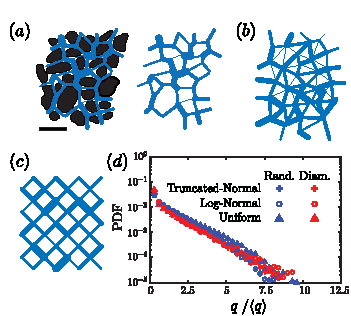
\includegraphics[width = 0.45\textwidth]{Figs/Fig1.eps}
    \caption{(a) An example of a porous media; (b) The real network of pores, and a structured grid equivalent case (c) The PDF of velocities for various distribution of diameters.}\label{fig:fig1}
\end{figure}


\section{Methods}
%
Flow through pores and throats of a porous medium can be modeled using a network of tubes with varying radii ( Fig. \ref{fig:fig1}a,b). In this network, the pores are represented with nodes, and the throats are modeled as simple tubes where the diameters/length can be random. where they approximate the flow resistance between the pores. A structured network of nodes with a random distribution of flow resistances for edges has shown to be a valid approximate model that correctly captures the exponential distribution of velocities of a porous medium. Here we consider this similar model to obtain some insights of structural change effects. We consider a fluid with density $\rho$ and kinematic viscosity $\mu$ flowing through the pores. We consider low Reynolds fluid or Poiseuille flow. In each tube Darcy's law hold $ P_i - P_j  = \frac{128 \mu L_{ij} }{\pi d_{ij}^4} Q_{ij}$ where $P_i,P_j$ represents pressures at pores $i,j$, and $d_{ij}, L_{ij}, Q_{ij}$ are respectively the radius, length, and fluid flow rate in the tube connecting pores $i$ and $j$. We then consider a network grid and assume a pressure difference between nodes left and the right boundary. Due to conservation of mass at each node, the total flow into a node should add up to zero. Solving for conservation of mass at all nodes, a system of equations can be obtained, where the solution is the pressures at all nodes. Using pressure values at the nodes, the flow rate in each tube is then obtained using Darcy's law. Considering different distribution of radius/length of the tubes, we find that the for any distribution, with large enough disorder the distribution of normalized fluid flux in the tubes collapses on a universal curve where $P(\hat{q}) \propto e^{-\alpha \hat{q}}$ for large $\hat{q}$ where $\hat{q}$ is the normalized fluid flux $\hat{q} = {q}/\langle q \rangle$. This can be simply proved using a mean field approximation (See supp material). 






\newpage
% Fig.2: network evolution for different parameters powers of n
\onecolumngrid
\begin{figure*}[h]
    % \centering
    \includegraphics[width = 1\textwidth]{Figs/ErosionSim.png}
    \caption{Erosion  simulations on a grid and a random network. (a)On a triangular grid network, we initialize every tube with a random radius uniformly distributed. The flow distribution is indicated by line width and transparency, the color gradient indicates the pressure field from the high pressure at the left boundary (red) to the low pressure at the right boundary (blue). (b) Different final states after 300 times iteration of erosion cases with different $n$'s. Channeling and homogenization are obvious in $n=1$ case and $n=6$ case respectively. The transition happens at $n=3$, which does not change the flow density distribution horizontally. (c) With the same number of points in the grid network, the position of every point is uniformly randomly distributed and we create the network using Delaunay triangulation to avoid crossed tube in 2D graph. Random radius is then assigned to every tube. (d) Different final states after 300 times iteration of erosion cases with different $n$'s. Similar channeling and homogenization effect are observed for $n=1$ and $n=6$ respectively. The transition happens at $n=3$, which does not change the flow density distribution horizontally.    }
    \label{fig:ErosionFig}
\end{figure*}

\twocolumngrid
% Fig 3: toy model
% Fig 4: phase transition



\section{Results}
\subsection{Simulation results for grid networks and random networks}
We run simulations on grid networks and random 2D networks. Both show similar results. For erosion cases, $n=3$ is a critical point that the final states will retain the exponential tail of flow distribution. When $n<3$, the erosion law yields channelling effect which strengthens a few tube faster than the rest. When $n>3$, the 
\section{Conclusion}

\bibliography{ref.bib}

\end{document}
%